%نام و نام خانوادگی:
%شماره دانشجویی: 
\مسئله{}

\پاسخ{}
الف) در زیر شکل vtable و ObjectLayout برای شیء SUV کشیده شده است:
\graphicspath{{./images/}}
\begin{center}
	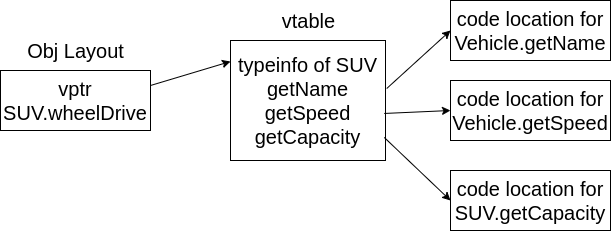
\includegraphics[scale=0.7]{Q4_1.png}
\end{center}
حال کمی آن را توضیح می‌دهم.\\
در سمت چپ شکل ObjectLayout را داریم که در خانه اول آن اشاره‌گر به vtable قرار دارد و در خانه دوم آن مقدار متغیر SUV.wheelDrive ذخیره شده است.
در وسط vtable قرار دارد. در خانه اول آن typeinfo مربوط به کلاس SUV قرار دارد و در ۳ خانه بعدی اشاره‌گرهای به کدهای همه توابع قرار دارد.\\\\
ب) در زیر شکل  vtable ها و ObjectLayout برای شیء BMW وجود دارد. دقت شود که با این‌که اشاره‌گر از نوع Drivable هست، اما به هر حال شیء ساخته شده از نوع BMW خواهد بود و من هم اجزاء آن را رسم کرده‌ام:
\graphicspath{{./images/}}
\begin{center}
	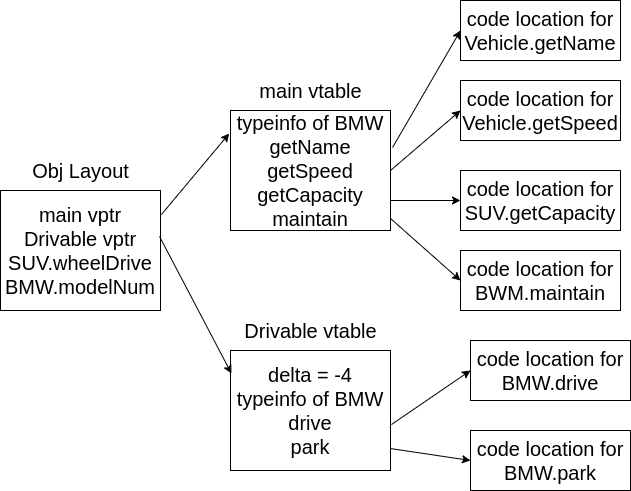
\includegraphics[scale=0.7]{Q4_2.png}
\end{center}
حال کمی آن را توضیح می‌دهم.\\
در سمت چپ ObjectLayout وجود دارد که ۲ اشاره‌گر به vtable دارد. اولی یعنی vptr main به vtable ای اشاره می‌کند که توابع BMW و یا پدرش ( SUV و یا پدر آن یعنی Vehicle ) را در خود دارد. دومین اشاره‌‌گر یعنی vptr Drivable به vtable ای اشاره می‌کند که توابع  اینترفیس Drivable را دارد. دقت شود که باید مقدار delta را هم مشخص می‌کردیم که در اینجا منفی ۴ هست.
